\subsection{Period 2: Drop and disappearance of the main haze layer around the Vernal Equinox (2008-2012) - $L_s=\ang{340}-\ang{30}$}

A precursor sign of the drop of the detached haze can be seen in March 2008 (Fig.~\ref{fig:dhl_2008_2012}a).
The main haze starts an initial contraction, perceptible around \ang{35}S. There, the depleted zone is almost
75 km thick at its maximum. In January 2009, the main haze continued to fall down from 425 km down to 375 km
while the detached haze layer remained around 500 km (Fig.~\ref{fig:dhl_2008_2012}b). After the drop
of the main haze in early 2009, the detached haze starts its own descent in June 2009, just before the equinox
(Fig.~\ref{fig:dhl_2008_2012}c). This delay in collapse increased the apparent thickness of the depletion
zone between the two haze layers.

\begin{figure*}[!ht]
    \centering
    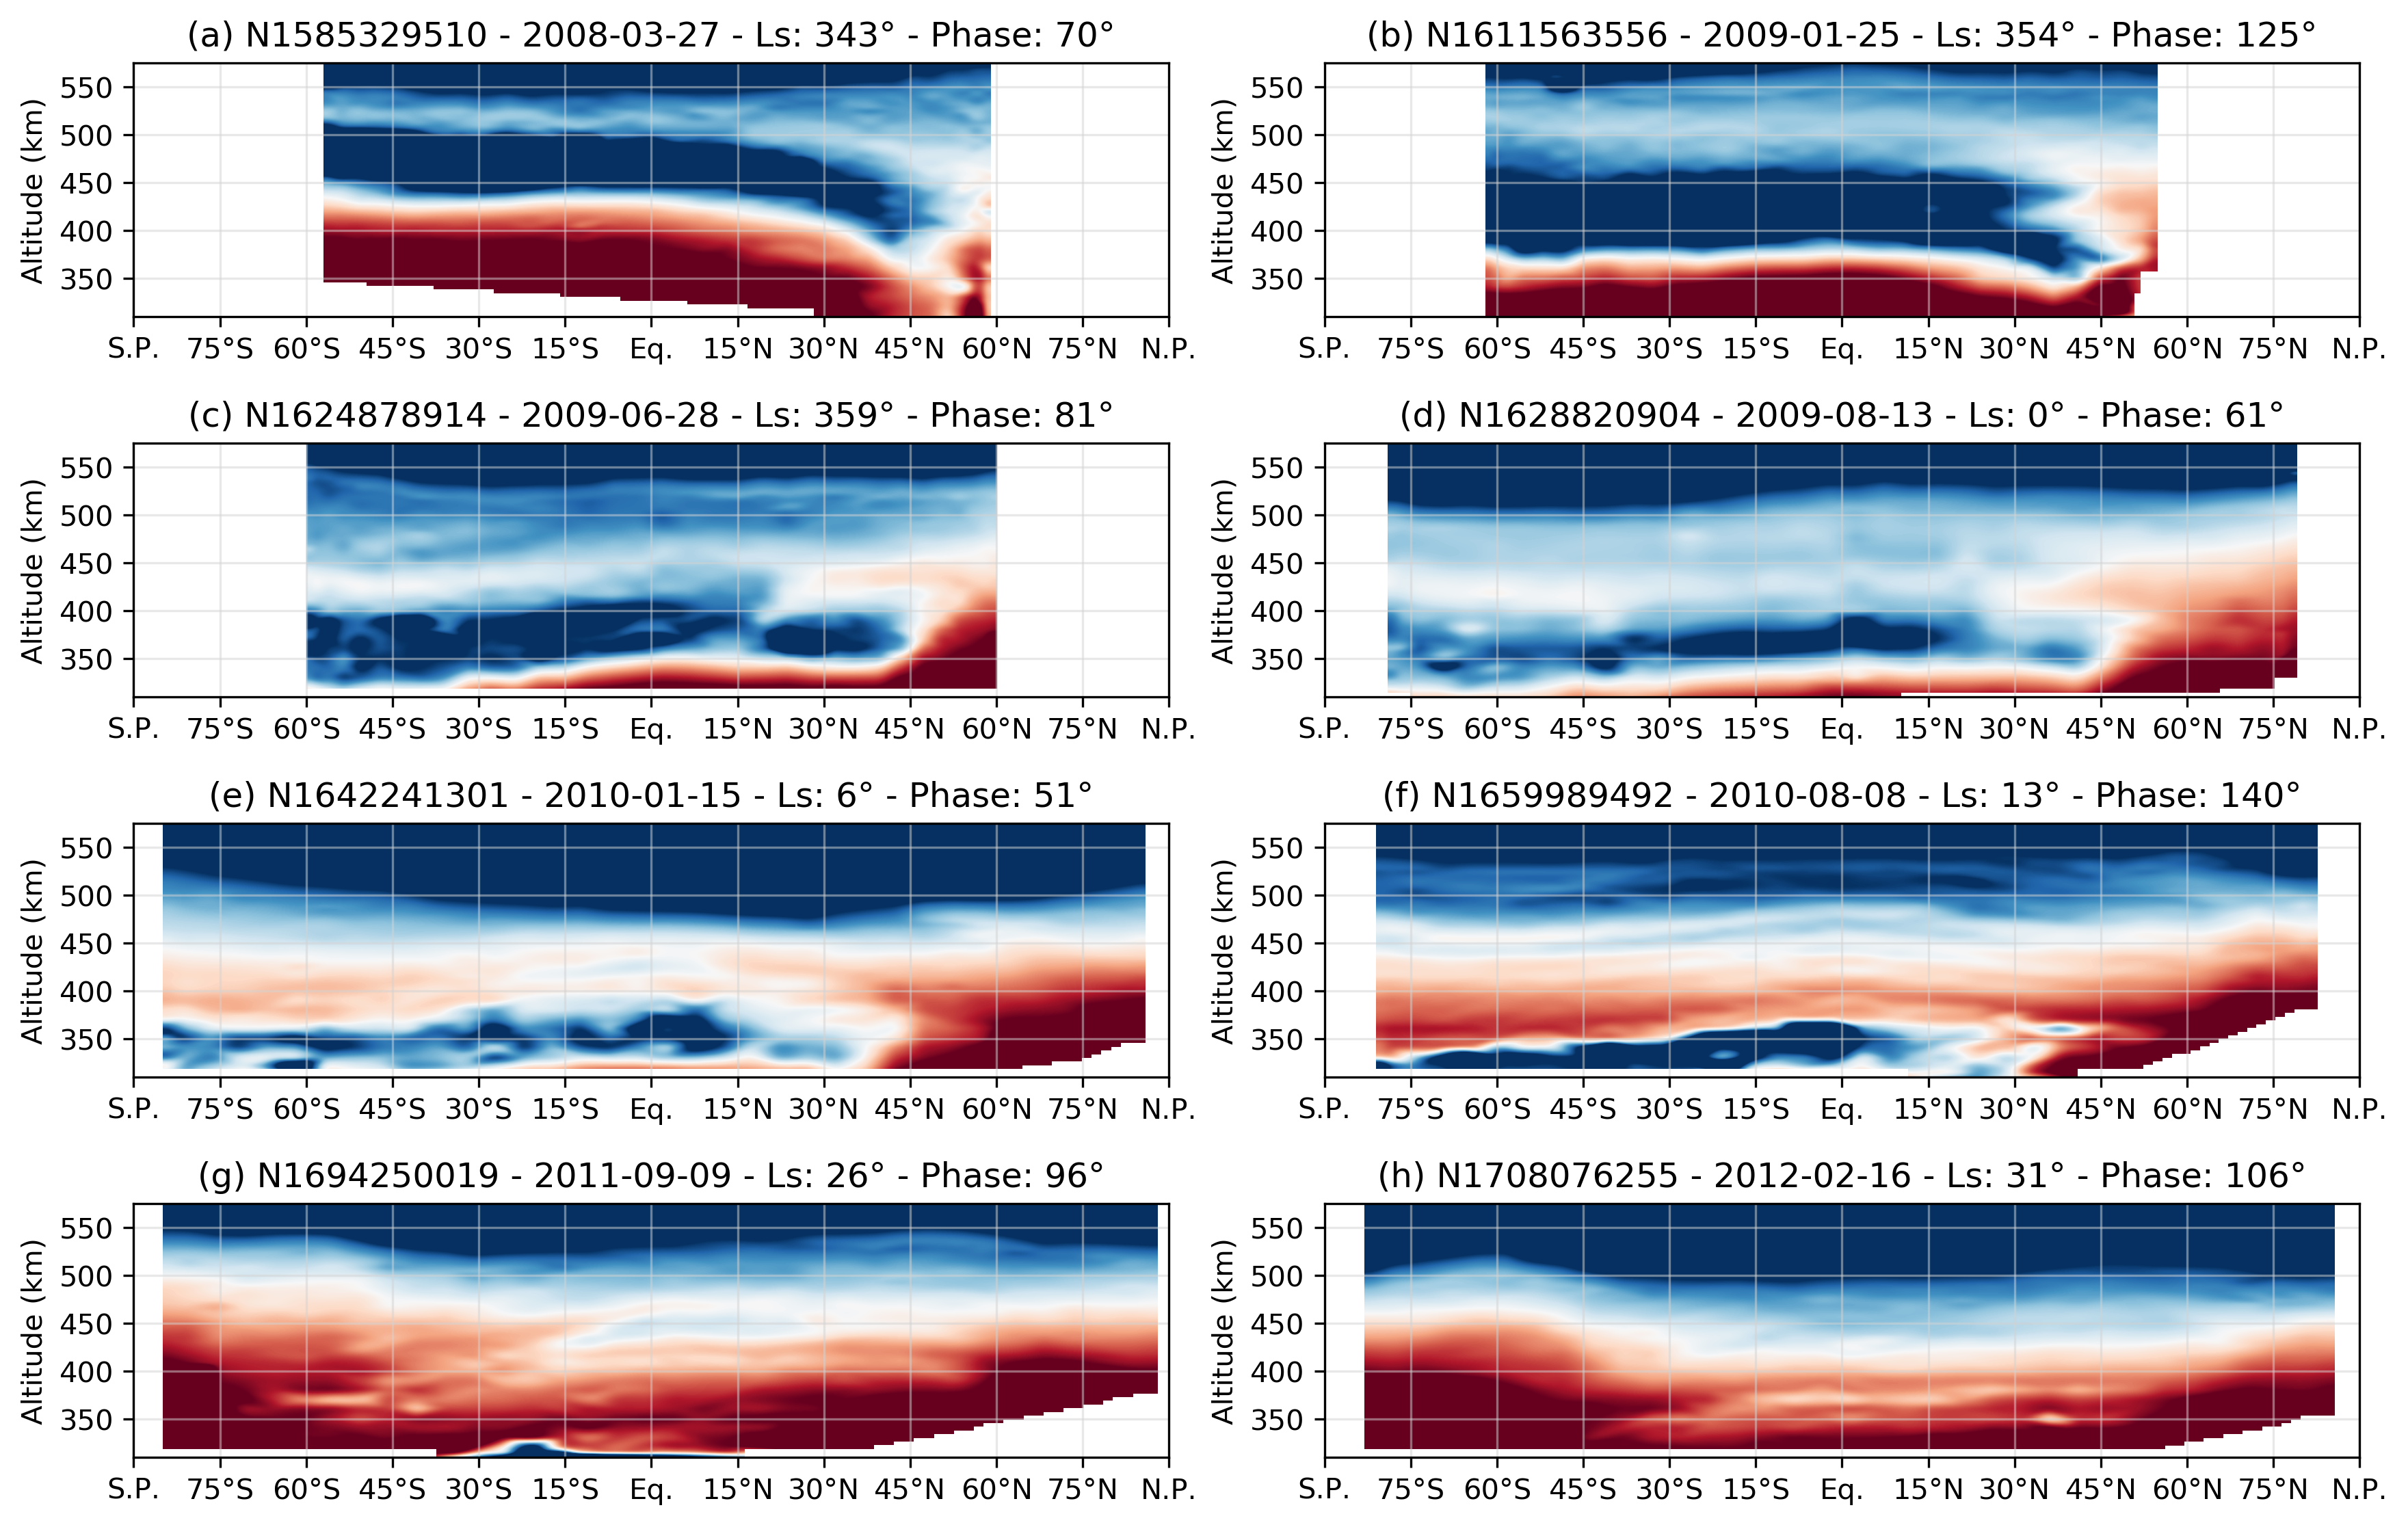
\includegraphics[width=\textwidth]{Fig/Lat_beta-2008_2012.png}
    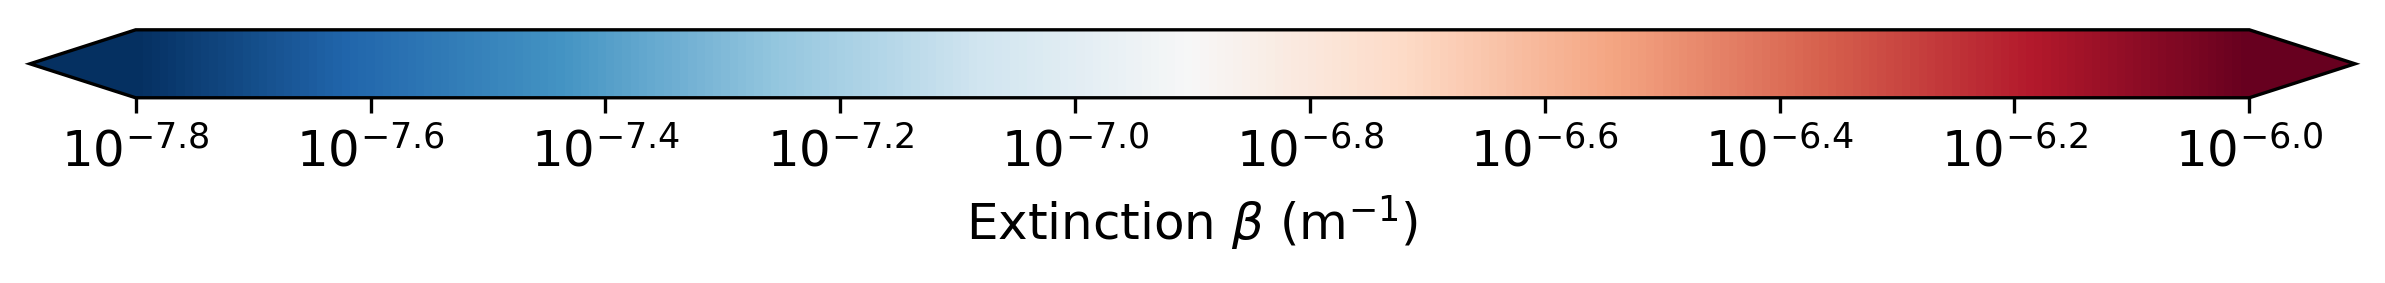
\includegraphics[width=.5\textwidth]{Fig/Extinction_colorbar.png}\vspace{-.3cm}
    \caption{Same as the figure~\ref{fig:dhl_2004_2008} for 8 images taken between 2008 and 2012
    ($L_s=\ang{340}-\ang{30}$) showing the drop and disappearance of the DHL.
    The color schema extent is kept similar to the figure~\ref{fig:dhl_2004_2008} to provide
    direct comparisons but the altitude range is extended down to 300 km around the UV3 saturation
    level (where the atmosphere is opaque).}
    \label{fig:dhl_2008_2012}
\end{figure*}

As for the main haze, the detached haze collapses first in the South hemisphere, from 500 km to 425 km, and
then at equator and in the northern hemisphere (Fig.~\ref{fig:dhl_2008_2012}c).
This is associated to the circulation turnover affecting first the summer hemisphere ascending branch.
With time, the detached haze gradually settled in altitude and finally merged with
the main haze. The complete collapse of the detached haze is displayed in Fig.~\ref{fig:dhl_2008_2012}c to
Fig.~\ref{fig:dhl_2008_2012}h. We note that the extinction of the detached haze is smaller at equator than at
other latitudes, and this will be the case during all the drop.

During the fall, a second thin detached haze layer, at planetary scale, can be remarked above the collapsing detached
haze layer. In January 2010 (Fig.~\ref{fig:dhl_2008_2012}e), the detached is now located between 375 and 400 km.
We can still see a double deck of haze, and this time the detached haze appears higher at the equator compare to the two
hemispheres, producing an arch. The haze extinction has globally increased by a factor of two due to sedimentation
in denser layers.

In August 2010 (Fig.~\ref{fig:dhl_2008_2012}f), one year after equinox, the detached haze layer continued
its drop down to 350 km around \ang{40}N and 400 km at the equator. It has gained in complexity with
multiple secondary layers up to 520 km. The detached haze form a remarkable arch with a difference of about 50 km
in altitude between the equator and the poles as previously noticed by~\cite{West2011}.
This observation and the next one correspond to the same time of the
year than the time of Voyagers flybys ($L_s=\ang{8}$ and \ang{18}). They can be compared quite directly. We now know
that this season was a time of rapid change, and that the Voyager probes observed transient situations. Voyager also
observed the detached haze higher near equator than elsewhere \citep{Rages1983, Rannou2000}. This corresponds to
the detached haze layer following an isobar level.

Due to orbital constrain and mission planning, the next observation was made in September 2011
(Fig.~\ref{fig:dhl_2008_2012}g). The detached haze layer is now well below the level of the polarhoods.
Again secondary detached layers show up as high as 470 and 520 km.
The south polarhood was not present in January 2010 (Fig.~\ref{fig:dhl_2008_2012}e), it could not be seen
neither northward to \ang{70}S in August 2010 (Fig.~\ref{fig:dhl_2008_2012}f). We conclude that it was surely
built in less than 20 months, and may be less than seven months. The circulation started to reverse around the equinox
and the southward circulation send haze in the south pole and produced this polarhood. The change in haze distribution
is a very good indication of the timing of the equinoctial circulation turnover, has it is discussed later. We note
that the strong haze depletion at 300 km and between \ang{30}S and \ang{20}N is real but may be exaggerated at \ang{20}N
due to the limit of the retrieval procedure. At this altitude level, Titan's atmosphere is opaque to UV radiations
(see Fig.~\ref{fig:model_uncertainties}) and does not allow use to follow the main depletion below this altitude.
ISS observations made with the Blue and Green filters seem to show that the main DHL continues
its descend below 300 km during 2011. Since our current model was only tested for UV observations, we were not able
to observe its merge with main haze.

The last image UV3 that we have with a detached is February 2012 (Fig.~\ref{fig:dhl_2008_2012}h). At that
time, the initial detached haze has completely disappeared and the secondary detached hazes is still descending
and reach 400 km. The secondary detached hazes is not well delineated by a layer strongly depleted in aerosols.
The south polarhood increases its latitudinal extent northward to \ang{50}S and becomes larger than the northern
polarhood which tends to decrease.
